\documentclass{article}
\usepackage{pdfpages}

\title{Team Liza \\ Milestone 4}
\author{Sam Kim \\ Kevin Geisler \\ Michael Williamson \\ Brian Collins}
\date{1-26-12}

\begin{document}

\maketitle
\newpage

\tableofcontents

\newpage

\section{Domain Model}

The domain model did not change due to the Grasp principles.  Although some 
changes were made in the DCD, this did not require the Domain model to change.
This is because the additional classes will be used in the testcode class in the 
Domain Model.  The communication will continue to work as the diagram depicts below:

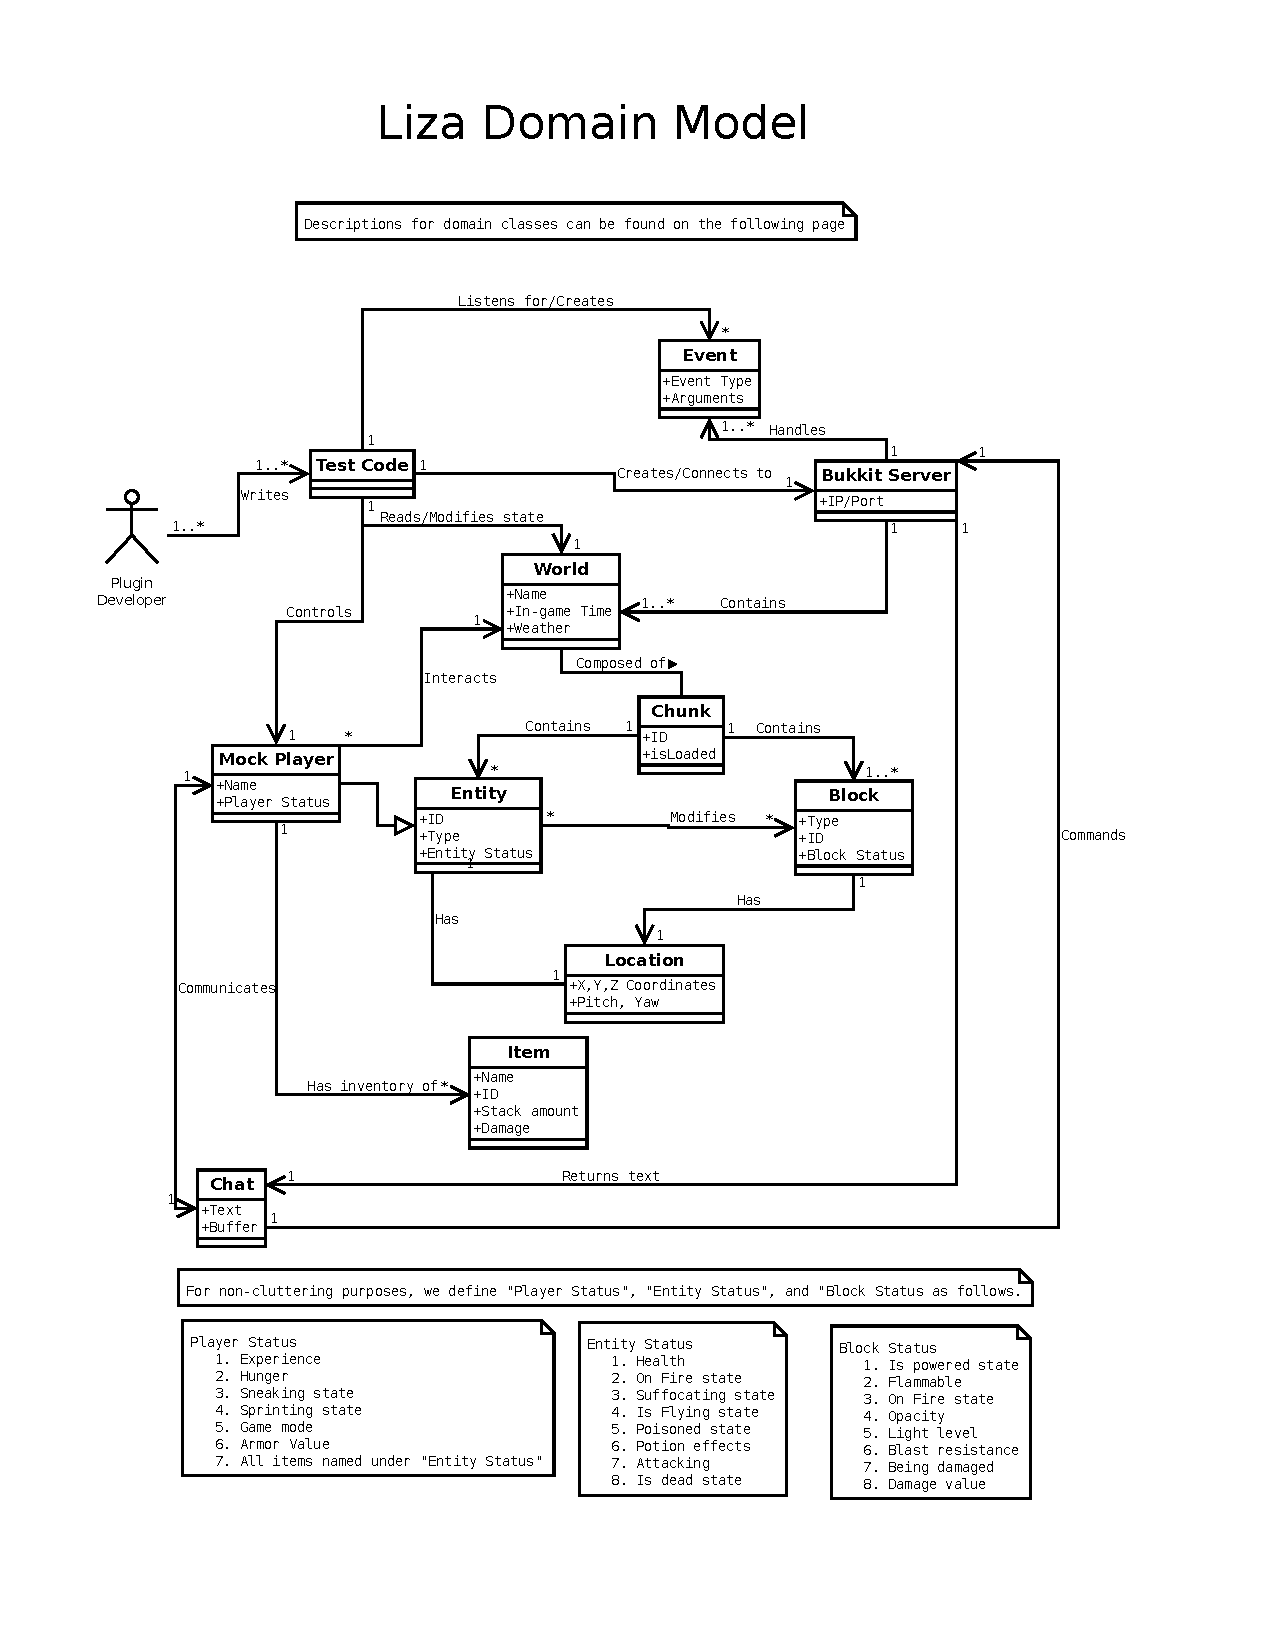
\includepdf[pages={-}]{DomainModel.pdf}



\section{System Sequence Diagrams (SSD)}

Description:  \newline

There are many SSDs that will apply to this project -- one for each assertion. 
However, each of these will follow the exact same format. Instead, we
produced a single SSD that details the flow of a test case that a developer may
write.  This includes general exception cases and alternate paths which could be
produced.  \newline 



Even though we have many SSD's in our design, most of the user interation revoles 
around the test code and the API that will be provided by the API.  Due to this, our 
general case SSD did not change.

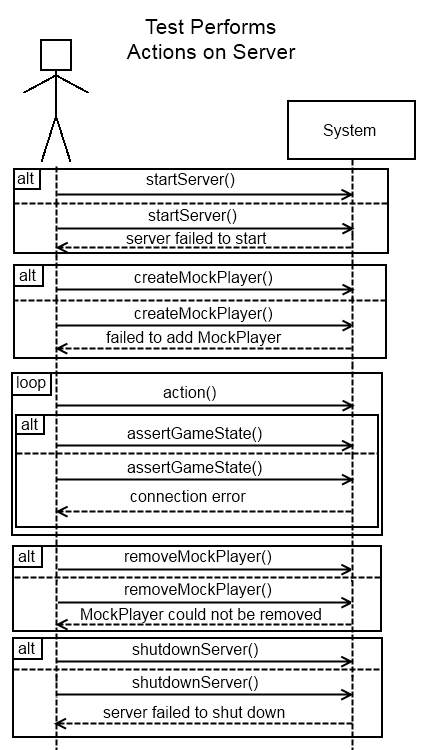
\includegraphics{ssd}

\section{Operational Contracts (OC)}

There will be a controller in Liza to start the server that it will control.
 Here is an operational contract which describes the startup process.:  \newline

\textbf{Operation name:} startServer() 
\newline \indent
\textbf{Cross-References:} SSD1 
\newline  \indent
\textbf{Preconditions:} LizaCraftController has been created.
\newline  \indent
\textbf{Postconditions: }
	\begin{enumerate}
		\item CraftBukkitThread was created.
		\item CraftBukkitThread was run
		\item CraftServer object was retrieved from CraftBukkitThread
		\item EventListener was created
		\item Association between EventListener and CraftServer established
	\end{enumerate}•

\section{Package Diagram}

There exists a degree of separation between our system and Bukkit, in the
sense that our system interacts with Bukkit, yet Bukkit is not aware of our
system. However, all of the classes in our system will all belong to the same
package, due to the high amount of interaction between classes. Because
of this, a package diagram is not applicable.  However, we have included a 
diagram which depicts the relationship between Liza and Bukkit in general.
For each Bukkit class that is relavent, Liza will extend a new interface and 
create a new LizaCraft class that will implement it. \newline 

\noindent This relationship will not change due to the Grasp principles.  However, it is important to 
note that these relationships follow the protected variation design pattern.  This protects the Liza
package from the Bukkit Server.  This means that if the bukkit framework changes, that Liza will not be adversly
affected.  However, the draw back to this is that this design supports high coupling.  This taken into account there
is no way to have a separte testing framework without this effect.

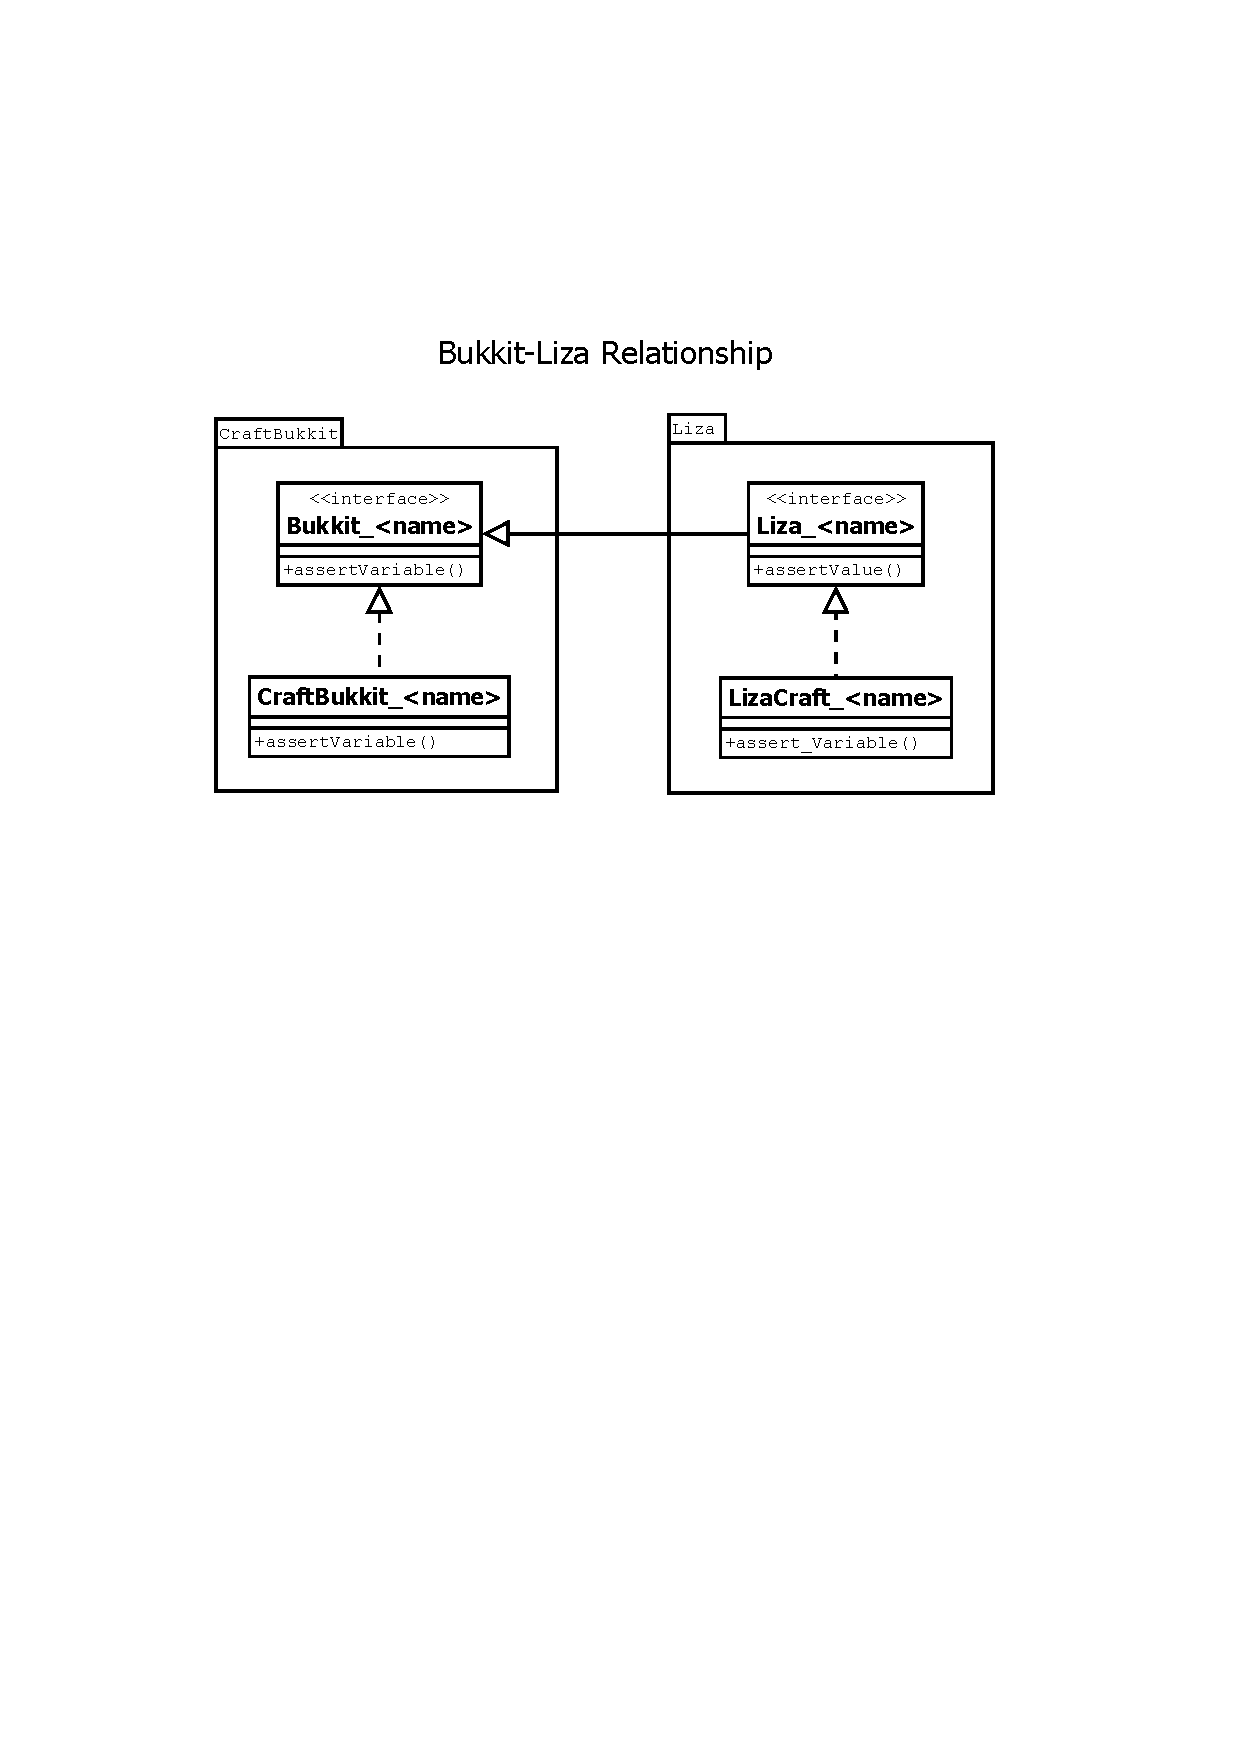
\includepdf[pages={-}]{Bukkit-Liza-Relationship.pdf}

\section{Class Diagram}

Description:
\newline

\noindent
Bukkit has two main layers: Bukkit, which is a collection of interfaces that
a plugin developer utilizes, and CraftBukkit, which is the implementation
of those interfaces. Our system will mirror this design. There is Liza, which
is a set of interfaces that inherit the Bukkit interfaces, and LizaCraft, which
is the implementation of the Liza interfaces and extends the CraftBukkit classes.
By extending the existing Bukkit and CraftBukkit, we present the API that
the developers are accustomed to, along with any new methods that may
be of use for testing, such as asserting properties. 
\newline

\noindent
There are a few new classes, however. LizaMockPlayer and its associated
implementation represent the automated player that the developer
commands. LizaMockPlayer and LizaPlayer are separated because the
latter asserts properties of any player, while the former controls only
the automated player.
\newline

\noindent
LizaListener and LizaEventExecutor handle the listening and spoofing of
events, respectively. 
\newline

\noindent
Grasp Principles:
\newline

\noindent
The Liza Unit Testing Framework follows the protected variation design pattern as
described as in the Package Diagram with the included drawback of a highly coupled system.
Due to the nature of the relationship of our system with Bukkit and Minecraft our design is limited.
With our design restriction, this limits the ability to communicate to classes without going through
other classes.  It would nice to create a more low coupled system but we are restricted here. \newline 

\noindent
We have created a LizaCraftController following the Grasp controller principle.  This will allow for the developer 
to create one class which will create the craftserver and grab the thread of it.  At the same time the class will
contain the craftsever so that the developer will know where to go to interface with Liza.
\newline



The diagram is found on the following pages.
\newline

\newpage
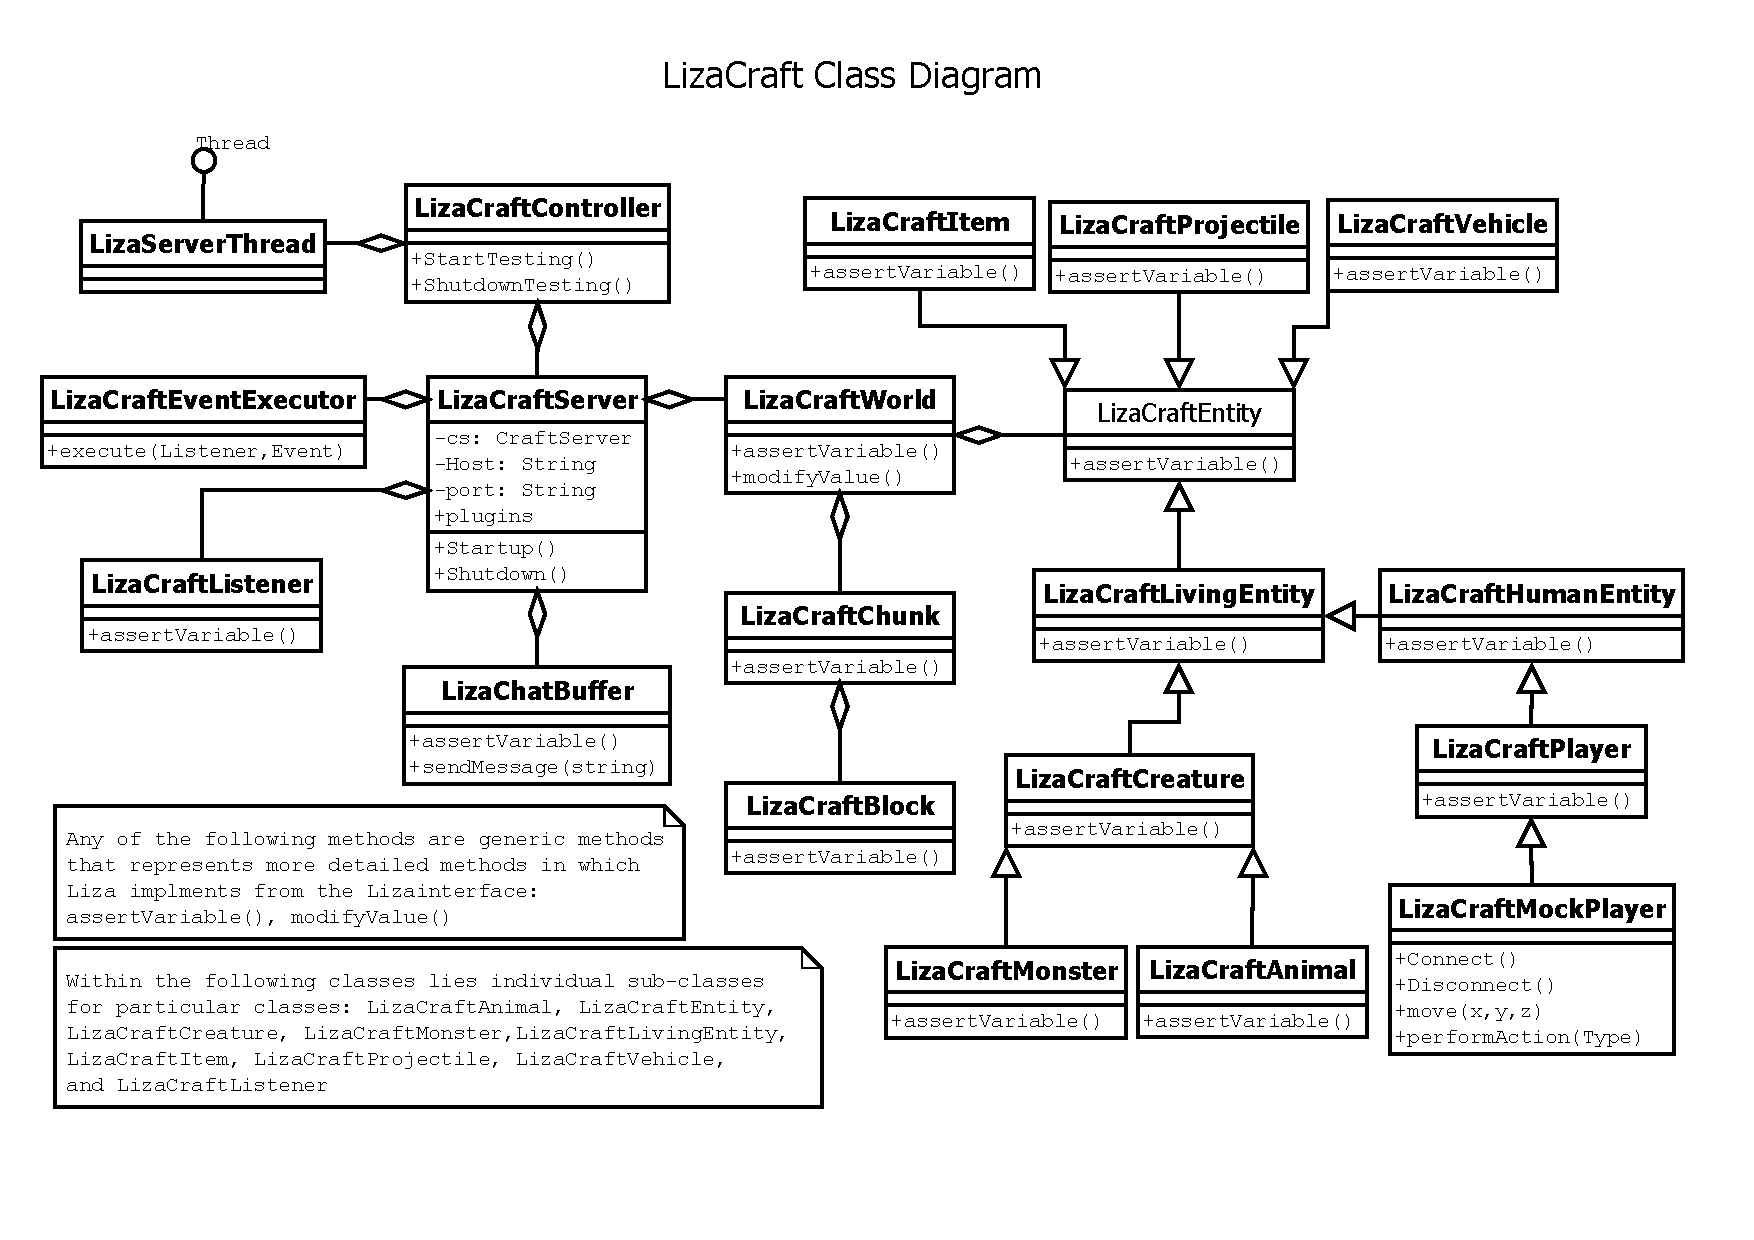
\includepdf[pages={-}]{LizaClassDiagram.pdf}

\newpage
\section{Application of GRASP Principles}

In previous sections, we have discussed some applications of GRASP principles. 
This section will reiterate those, and discuss others in detail.

	\subsection{Creator}

	Because our system mainly views the properties of an already running system,
	our code does not create many objects. However, we have a LizaController class.
	This class is responsible for creating the server thread object, retrieving the
	server, and creating the LizaListener.

	\subsection{Information Expert}

	This principle does not particularly apply to us. There is not very much data
	that goes through the system. Because of this, it is difficult to have an
	object be an ``expert''. The LizaController in its enabling of the EventListener
	may be seen as an information expert. In truth, the information needed
	is spread across many classes, but the LizaController sits at the top.

	\subsection{Controller}

	Once again, the LizaController, as the name suggests, is an application
	of a Use-Case Controller. It handles the flow of the beginning of the
	use-case, which is starting up and intializing the server and world. It
	may also include the creation of the Mock Players.

	\subsection{Low Coupling}

	Unfortunately, our system's architecture is highly reliant on that
	of Bukkit's. Bukkit (and Minecraft) is highly coupled, with countless
	numbers of circular references and dependencies. In order for our
	system to effectively work along Bukkit, we must share this coupling.

	\subsection{High Cohesion}

	Despite the high coupling, Bukkit's design is fairly cohesive. Each
	element of the game is put into its own class. As for Liza's implementation,
	the LizaController demonstrates higher cohesion, as
	starting up a server takes many steps across many classes. Putting this
	work into a single existing Bukkit class (such as the Server) would require
	responsibilities found in outside classes (such as PluginManager).

	The LizaPlayer and LizaMockPlayer was also an attempt to achieve higher
	cohesion. In addition to asserting states about a player, the system
	also needs to control an automated player. So control and assertion
	were split into two classes.

	\subsection{Polymorphism}

	As the class diagram shows, there is numerous cases of polymorphism, 
	which we inherit from Bukkit. The Entity class, in full, actually expands
	to roughly 60 classes in its heirarchy. 

	It is designed this way because Players should be able to interact
	with anything in the Minecraft world. However, different objects 
	may react in different ways. Therefore Polymorphism allows each
	object type to respond appropriately. 

	\subsection{Indirection}

	Each one of the LizaCraftObject classes is an application of
	Indirection. Each is composed of the matching CraftBukkitObject.
	This makes each LizaCraftObject class to act as an intermediary
	between the developer's test code and the Bukkit code.

	\subsection{Pure Fabrication}

	We do not believe that there are any ``pure'' applications of the
	Pure Fabrication principle, as in there aren't any objects that don't
	exist in the domain. However, some exist that are more of a ``side
	 effect'' of the means to implement some of the domain objects. 

	For example, the LizaListener isn't explicitly detailed in the domain
	model, but is a means of providing Events. Similarly, the LizaController
	isn't directly the ``Test Code'' found in the domain model. However,
	it begins and ends the process.

	\subsection{Protected Variation}

	The LizaObject interfaces are applications of Protected Variation.
	They extend the BukkitObject interfaces, and therefore have
	all the methods. However, the implementations are handled
	via an adapter. Therefore, changes in Bukkit's code should not
	force changes to the plugin developer's test codes, but only
	on the adapter level.

\newpage
\section{Prototype}

The prototype for this milestone is currently availble on github online at

\noindent
https://github.com/geislekj/Liza

\end{document}